\begin{figure}
	\centering
	\begin{minipage}[t]{.4\textwidth}
		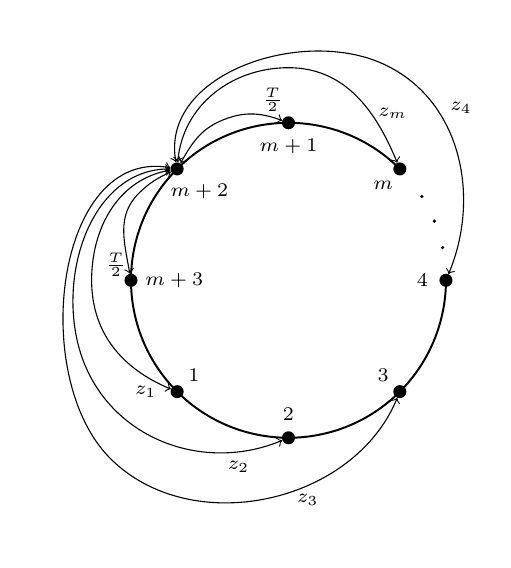
\begin{tikzpicture}[font=\scriptsize, node/.style={circle,thick,draw},
		l_2/.style={line width =0.25mm},
		scale=1, transform shape]
		% equidistant points and arc
		\foreach \x [count=\p] in {0,...,7} {
			\node[shape=circle,fill=black, scale=0.5] (\p) at (\x*45-135:2) {};
		};
		\foreach \x [count=\p] in {0,...,3} {
			\draw (225 + \x*45:1.7) node {\p};
			%				\draw (-30-\x*60:2.4) node {$\bar{\p}$};
		}; 
		\draw (225 + 4*45:1.7) node {$m$};
		\draw (225 + 5*45:1.7) node {$m+1$};
		\draw (225 + 6*45:1.6) node {$m+2$};
		\draw (225 + 7*45:1.45) node {$m+3$};
		
		\draw[l_2] (5) arc (45:360:2);
		\draw[line width =1.3pt, line cap=round, dash pattern=on 0pt off 10pt] (12:2) arc(12:35:2);
		

		\draw[<->] (1)  to [out=157.5,in=-90] (180:2.5) to [out=90,in=-170](7);
		\draw[<->] (2)  to [out=-157.5,in=-67.5] (-157.5:2.8) to [out=112.5,in=-180] (7);
		\draw[<->] (3)  to [out=-112.5,in=-45] (-135:3.2) to [out=135,in=-190] (7);
		\draw[<->] (4)  to [out=67.5,in=-22.5] (67.5:3) to [out=157.5,in=100] (7);
		\draw[<->] (5)  to [out=112.5,in=0] (90:2.7) to [out=180,in=85] (7);
		
		\draw[<->] (6)  to [out=160,in=22.5] (112.5:2.2) to [out=-157.5,in=60] (7);
		\draw[<->] (8)  to [out=100,in=-135] (150:2.2) to [out=45,in=-155] (7);
		
		\node (a) at (-142:2.3) {$z_1$};
		\node (b) at (-105:2.45) {$z_2$};
		\node (c) at (-85:2.8) {$z_3$};
		\node (d) at (45:3.1) {$z_4$};
		\node (e) at (58:2.5) {$z_m$};
		\node (d) at (95:2.3) {$\frac{T}{2}$};
		\node (f) at (175:2.2) {$\frac{T}{2}$};
%		\node (bottom) at (0, -2.8) {};
		%		\draw[dashed] (1) -- (3) -- (5) -- (1);
		% axes
		%		\draw [dotted, gray] (-2.6,0) -- (2.6,0);
		%		\draw [dotted, gray] (0,-2.15) -- (0,2.15);
		\end{tikzpicture}
	\end{minipage}
	\caption{\RL instance constructed from an instance of \textsc{Partition} consisting of naturals $z_1, \dots, z_m \in \N$.
	The demands are visualized as arrows between the respective nodes.}
	\label{fig:partition-rl-instance}
\end{figure}